\clearpage
\onecolumn
\setcounter{page}{1}
\journal{Supplementary Material}
\beginsupplement
\section*{Supplementary Material}

\begin{flushleft}
	\vspace*{1cm} % Force vertical space below header
	\textbf{\LARGE \papertitle} 
\end{flushleft}

% \author[1]{First \snm{Author}\corref{cor1}}
% \cortext[cor1]{Corresponding author: Address}
% \emailauthor{email@email.com}{First Author}


\begin{figure}[H]
	\centering
	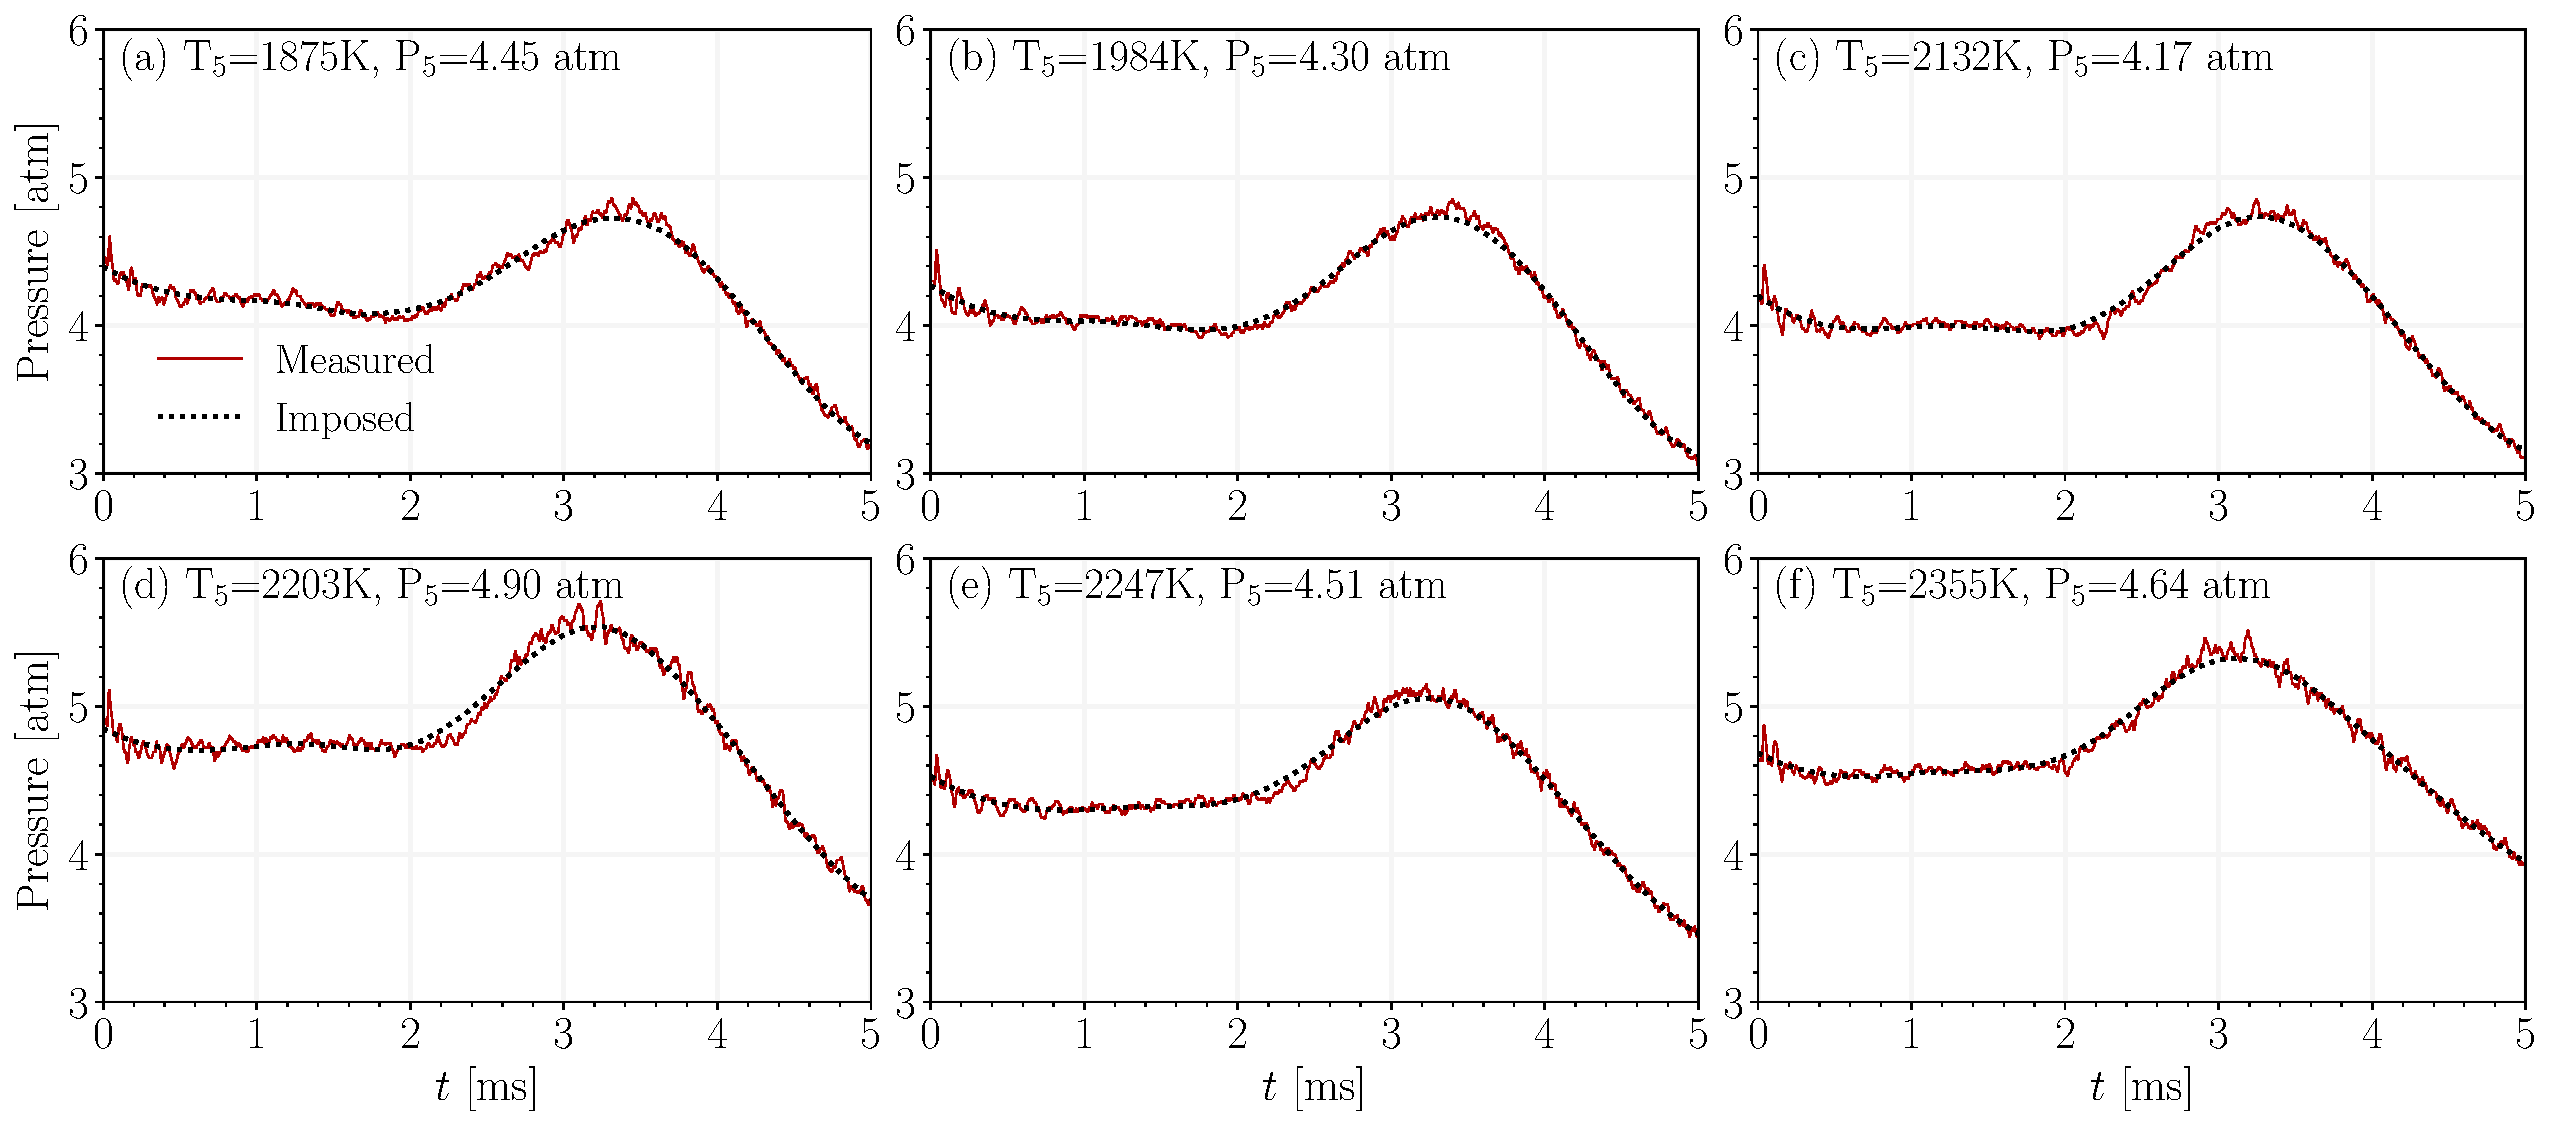
\includegraphics[width=0.85\textwidth]{Figures/pressure.pdf}
	\caption{The measure pressure trace and the filtered profile imposed in the model for the entire temperature range}
	\label{fig:pressureprofiles} 
\end{figure}


\begin{figure}[H]
	\centering
	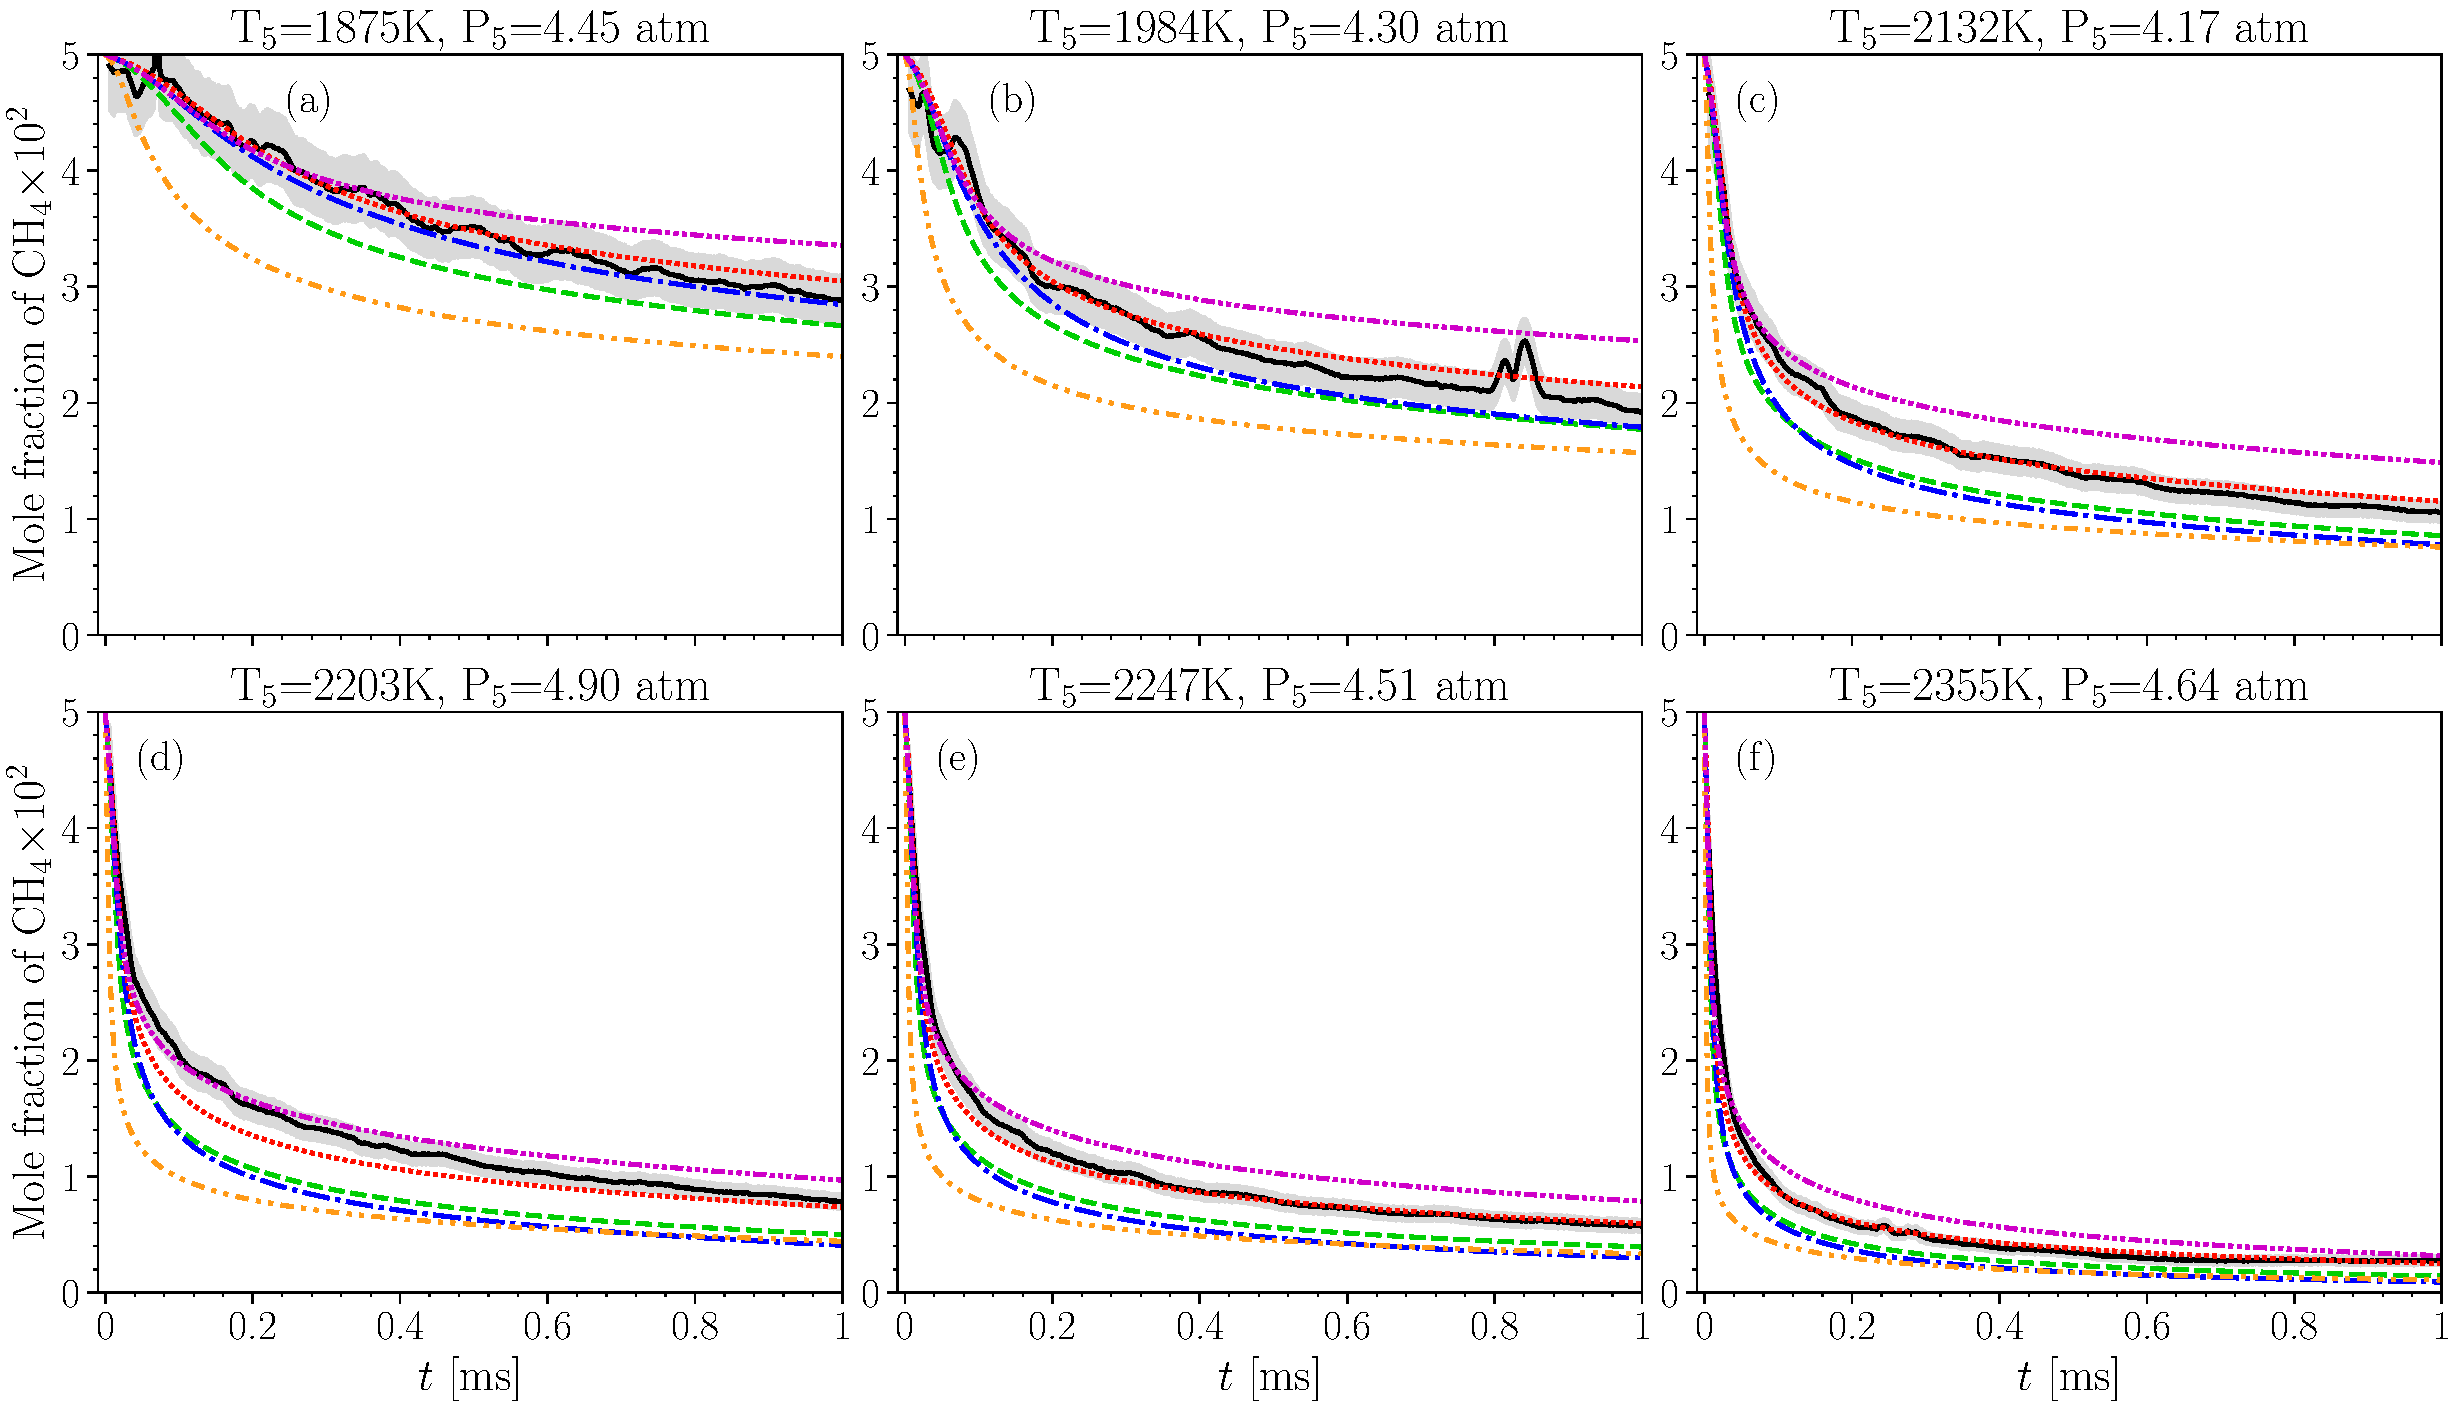
\includegraphics[width=0.85\textwidth]{Figures/CH4_all.pdf}
	\caption{The mole fraction time-history measurements of $\mathrm{CH_4}$ compared with the predictions of different kinetic mechanisms for $\mathrm{T_5}=1875$ (a), 1984 (b), 2132 (c), 2203 (d), 2247 (e), 2355~K (f). Shaded region around each measurement indicates experimental uncertainty.}
	\label{fig:ch4_all} 
\end{figure}

\begin{figure}[H]
	\centering
	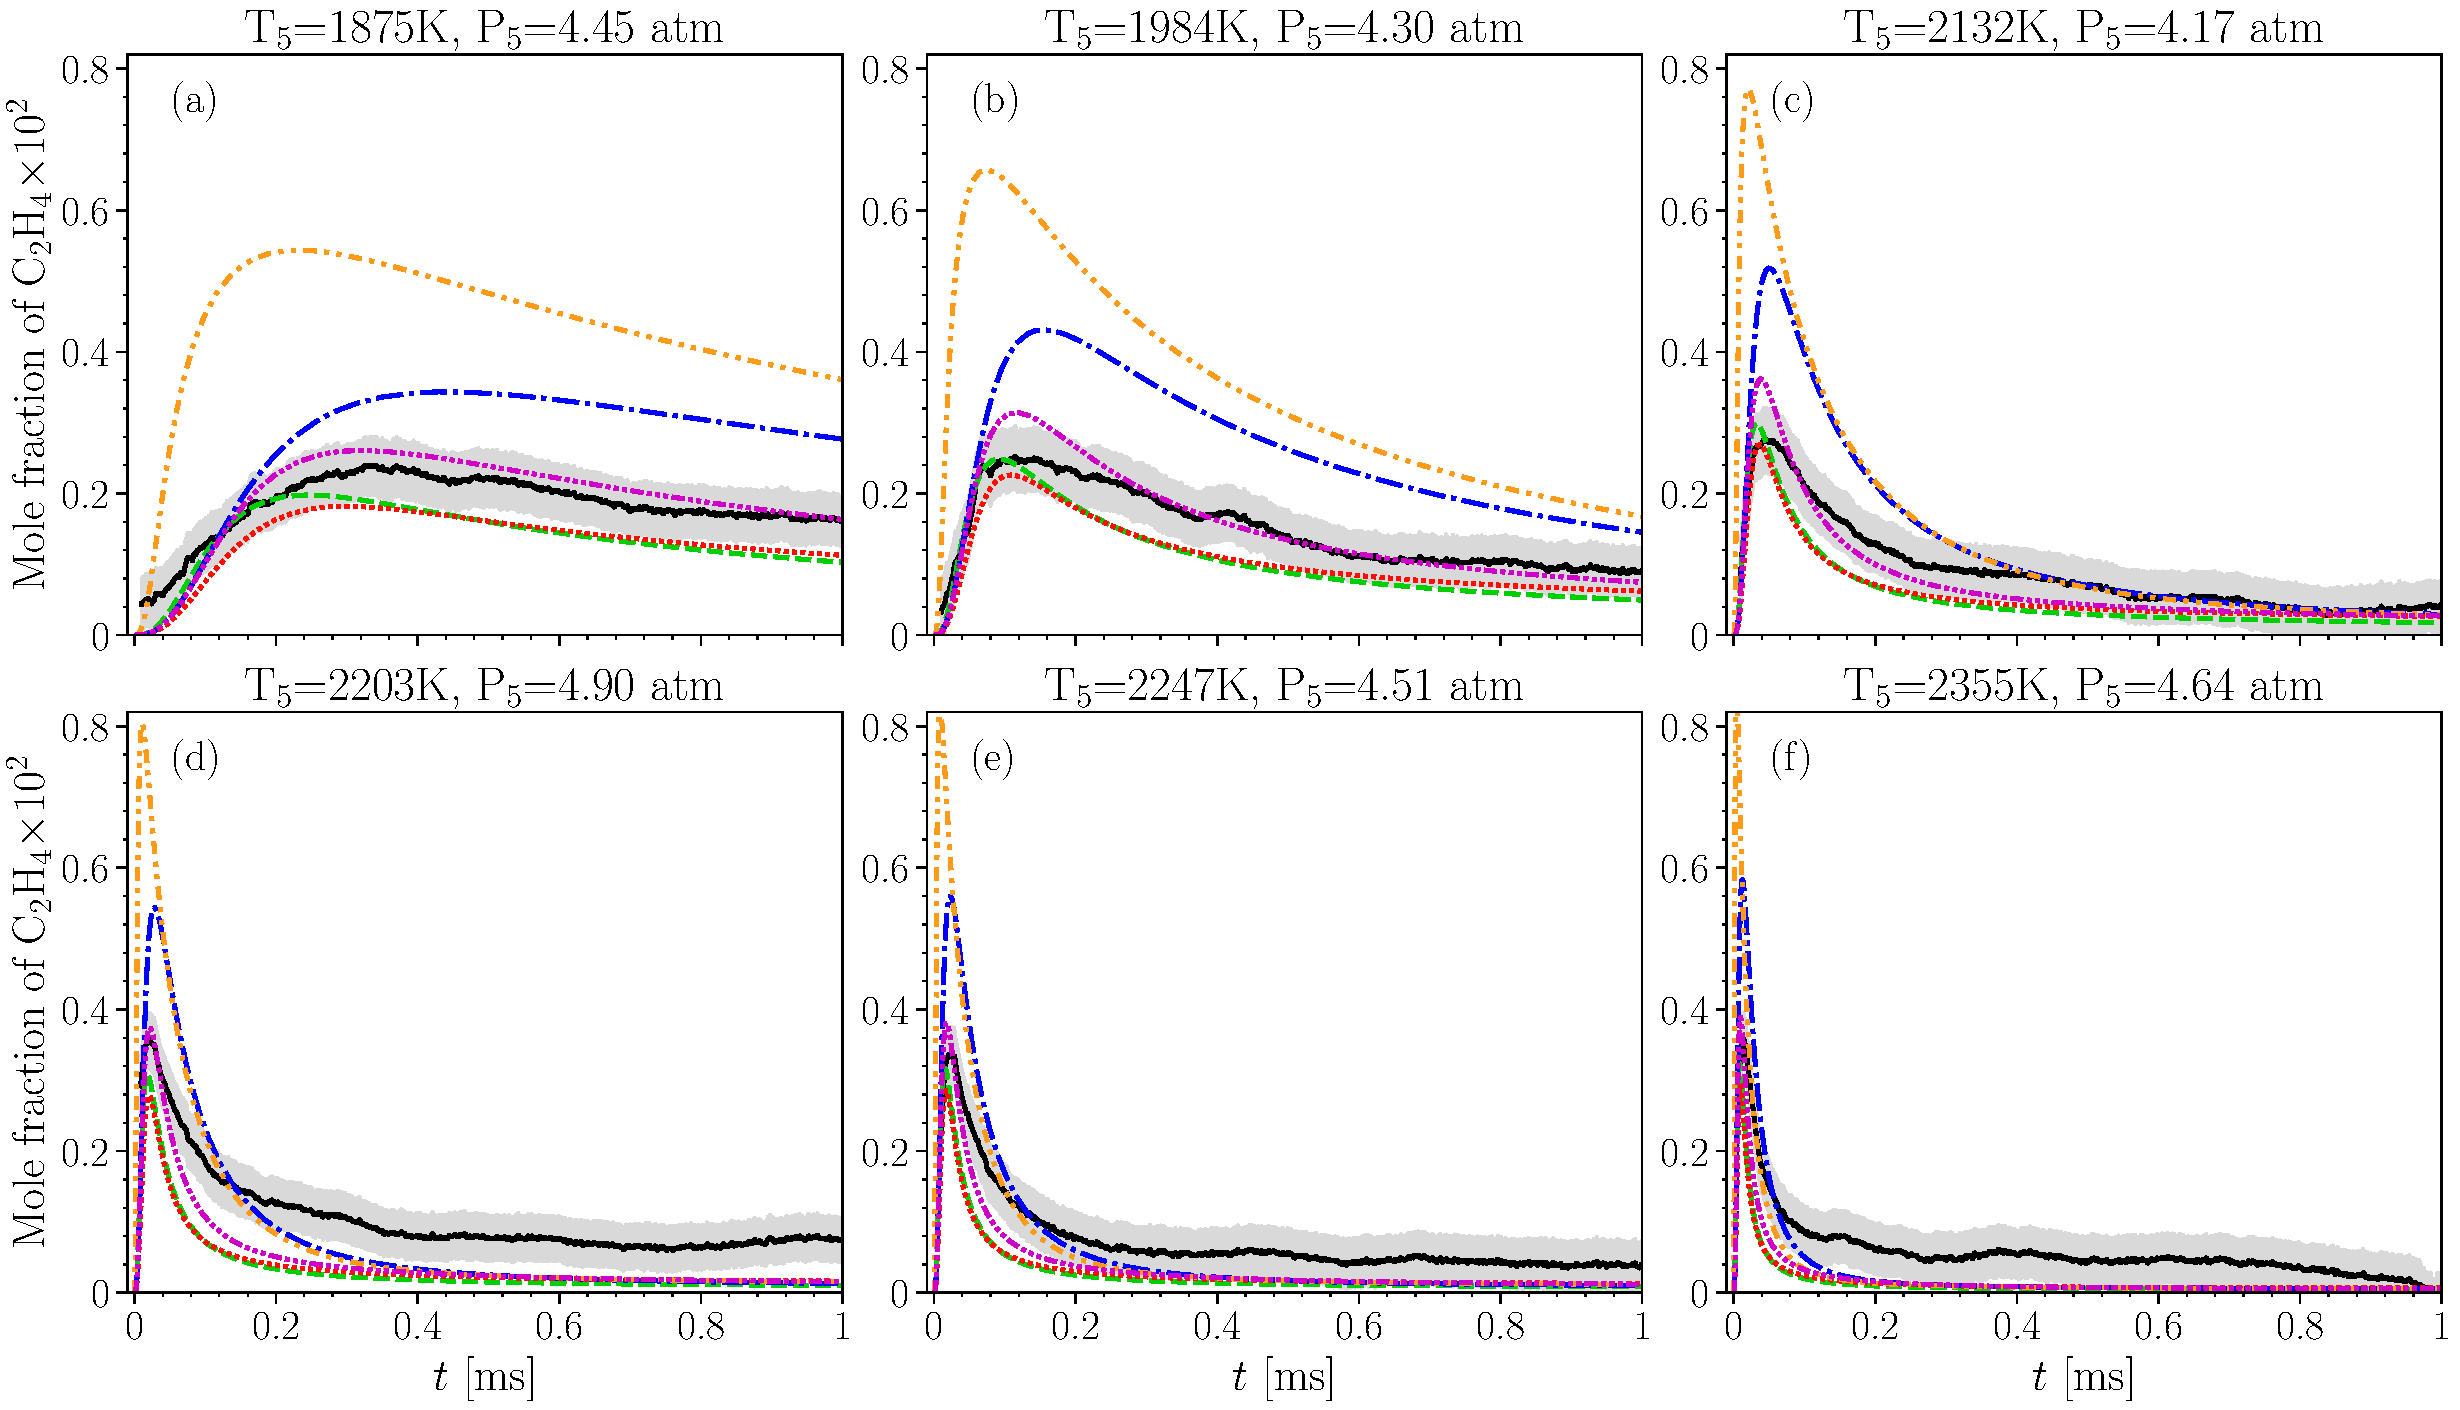
\includegraphics[width=0.85\textwidth]{Figures/C2H4_all.pdf}
	\caption{The mole fraction time-history measurements of $\mathrm{C_2H_4}$ compared with the predictions of different kinetic mechanisms for $\mathrm{T_5}=1984$~K and $\mathrm{T_5}=1875$ (a), 1984 (b), 2132 (c), 2203 (d), 2247 (e), 2355~K (f). Shaded region around each measurement indicates experimental uncertainty.}
	\label{fig:c2h4_all} 
\end{figure}

\begin{figure}[H]
	\centering
	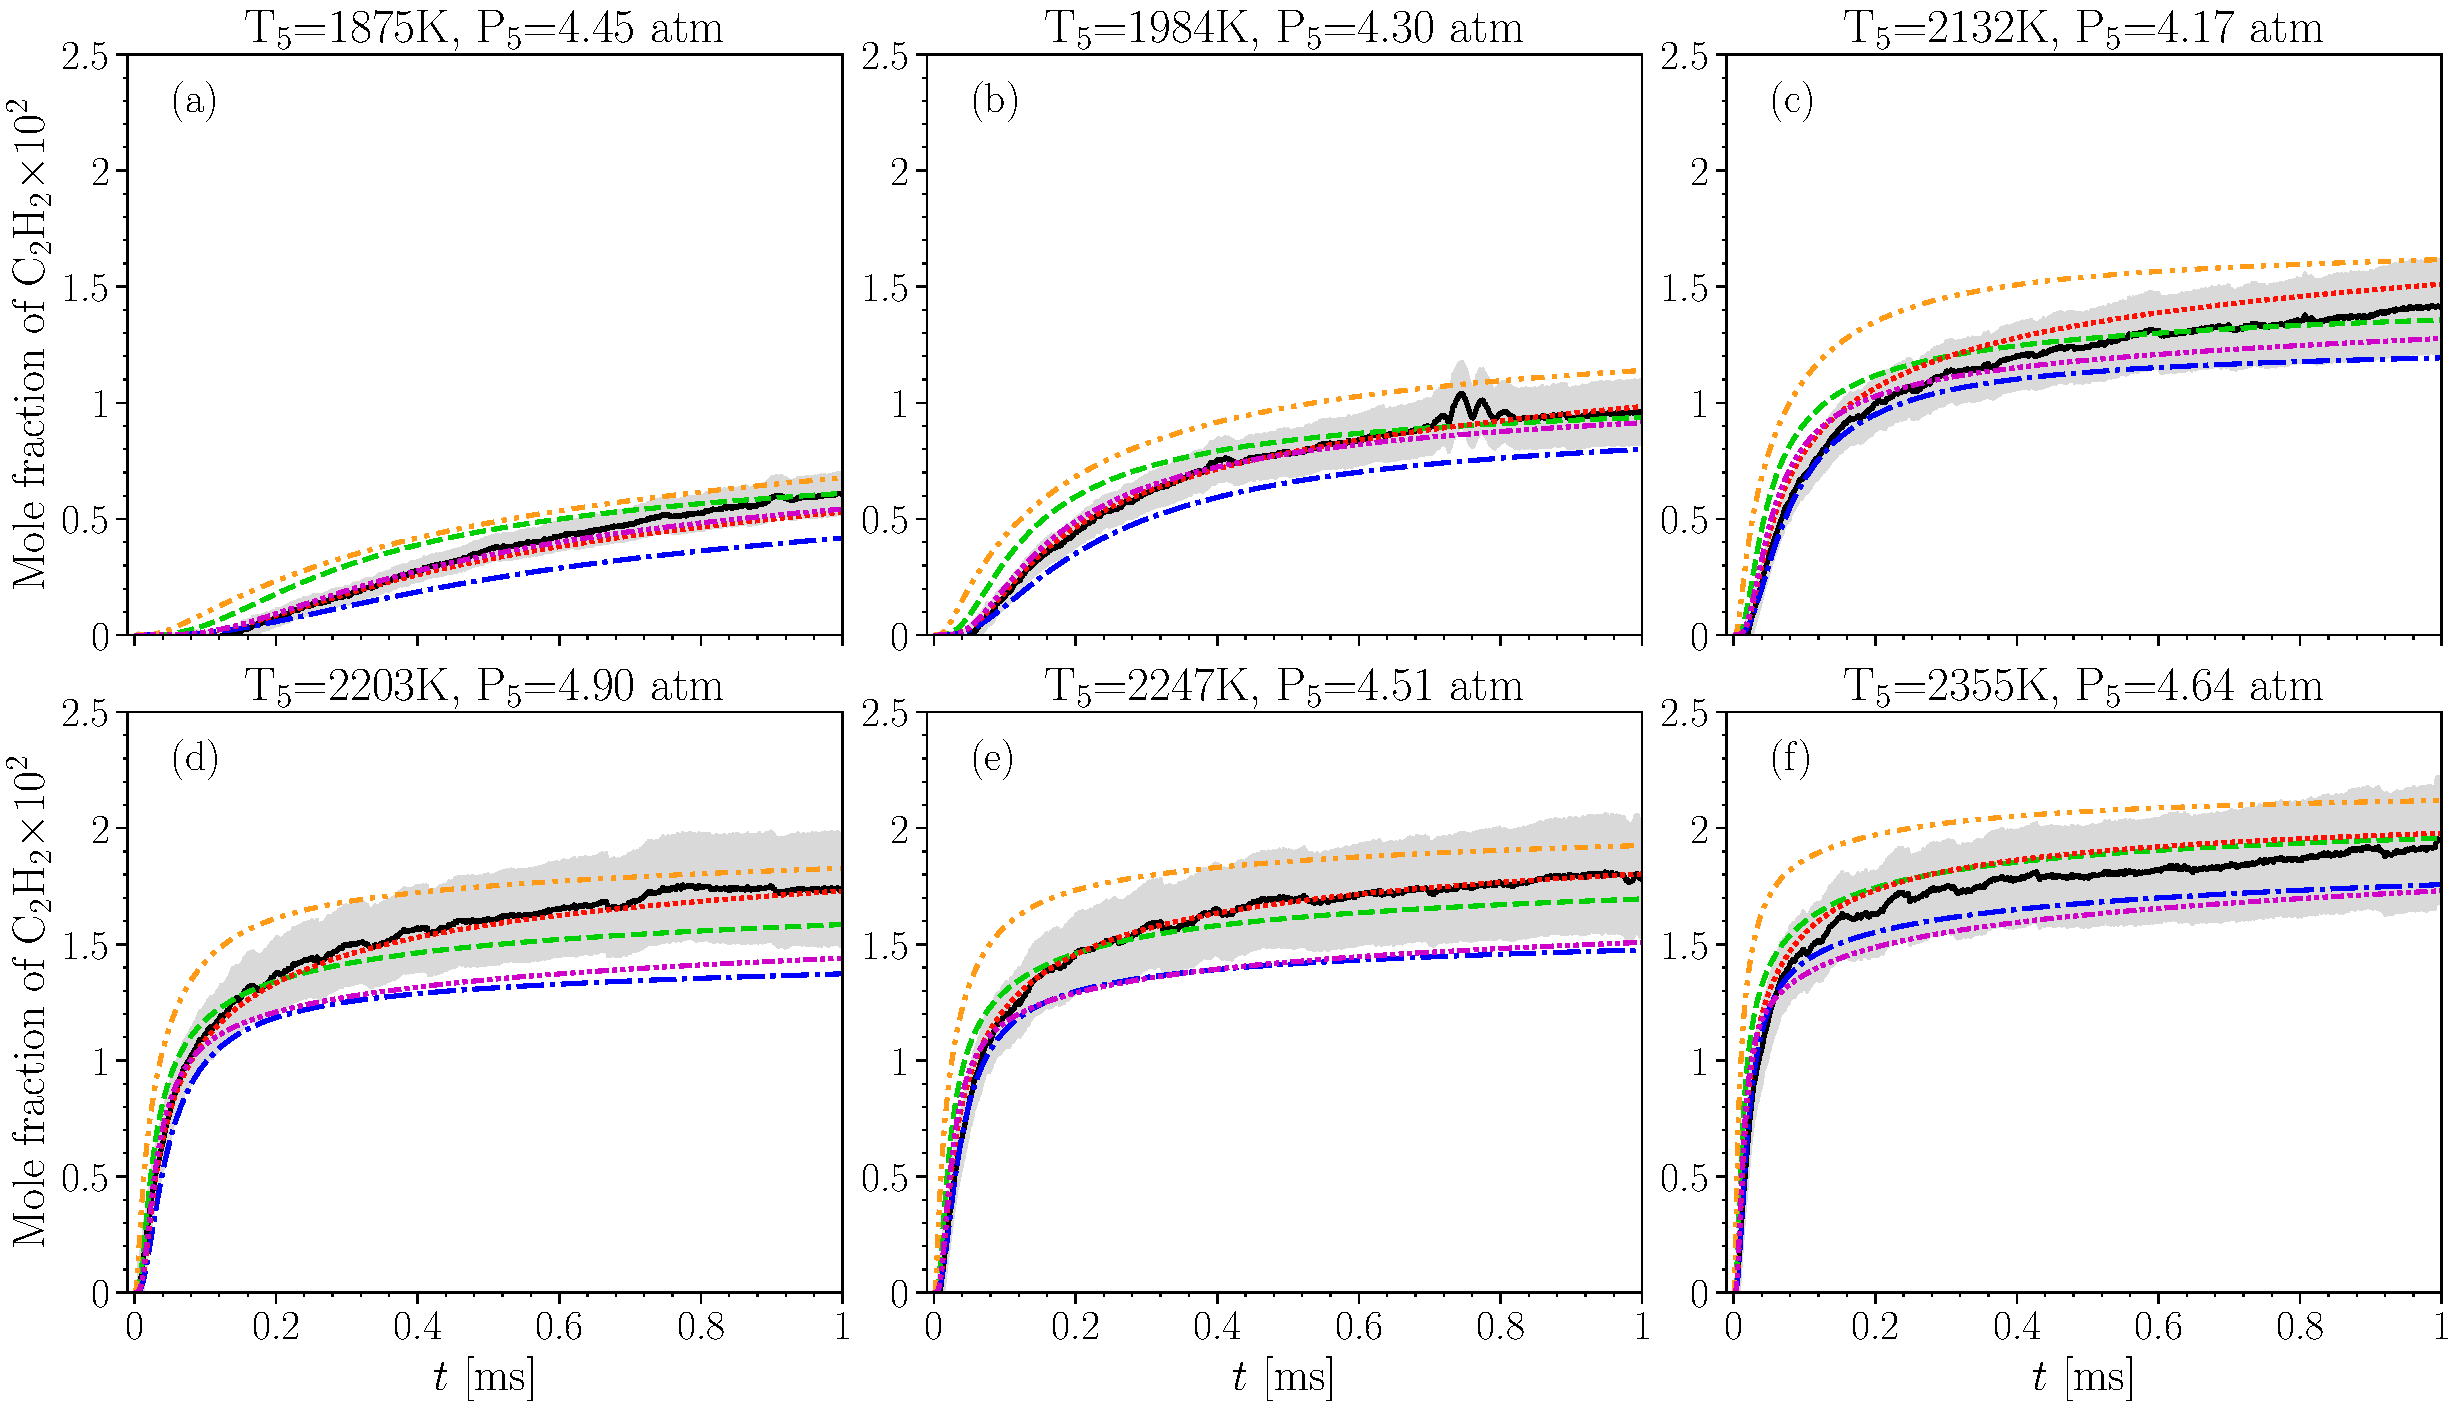
\includegraphics[width=0.85\textwidth]{Figures/C2H2_all.pdf}
	\caption{The mole fraction time-history measurements of $\mathrm{C_2H_2}$ compared with the predictions of different kinetic mechanisms for $\mathrm{T_5}=1984$~K and $\mathrm{T_5}=1875$ (a), 1984 (b), 2132 (c), 2203 (d), 2247 (e), 2355~K (f). Shaded region around each measurement indicates experimental uncertainty.}
	\label{fig:c2h2_all} 
\end{figure}


\begin{figure}[H]
    \centering
    \begin{subfigure}[t]{0.32\textwidth}
        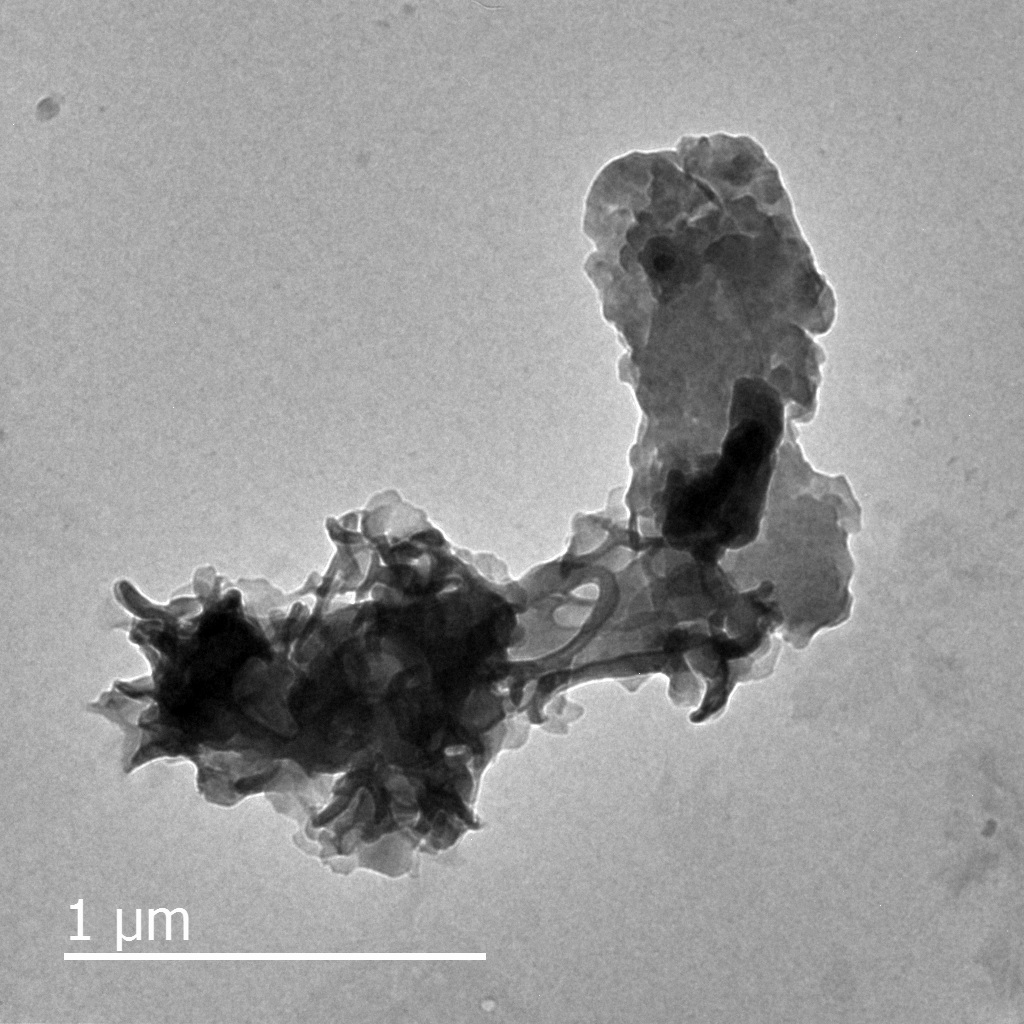
\includegraphics[width=1\textwidth]{Figures/1875K.jpg}
    \end{subfigure}
    \begin{subfigure}[t]{0.32\textwidth}
        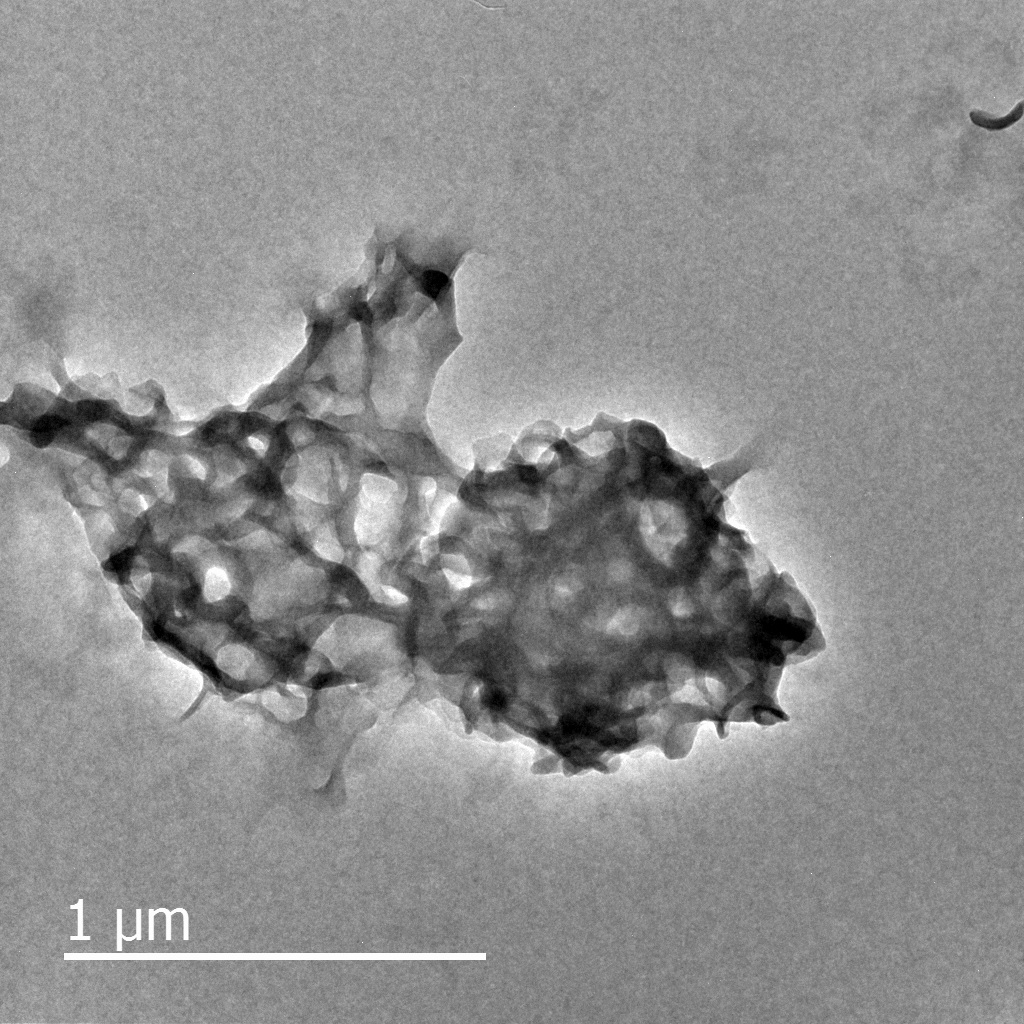
\includegraphics[width=1\textwidth]{Figures/1875K_2.jpg}
    \end{subfigure}
	\caption{Samples of TEM images collected for $\mathrm{T_5}$=1875~K that shows a compact carbonaceous lump with not clear boundaries between primary particles.}
	\label{fig:tem1875} 
\end{figure}

\begin{figure}[H]
	\centering
	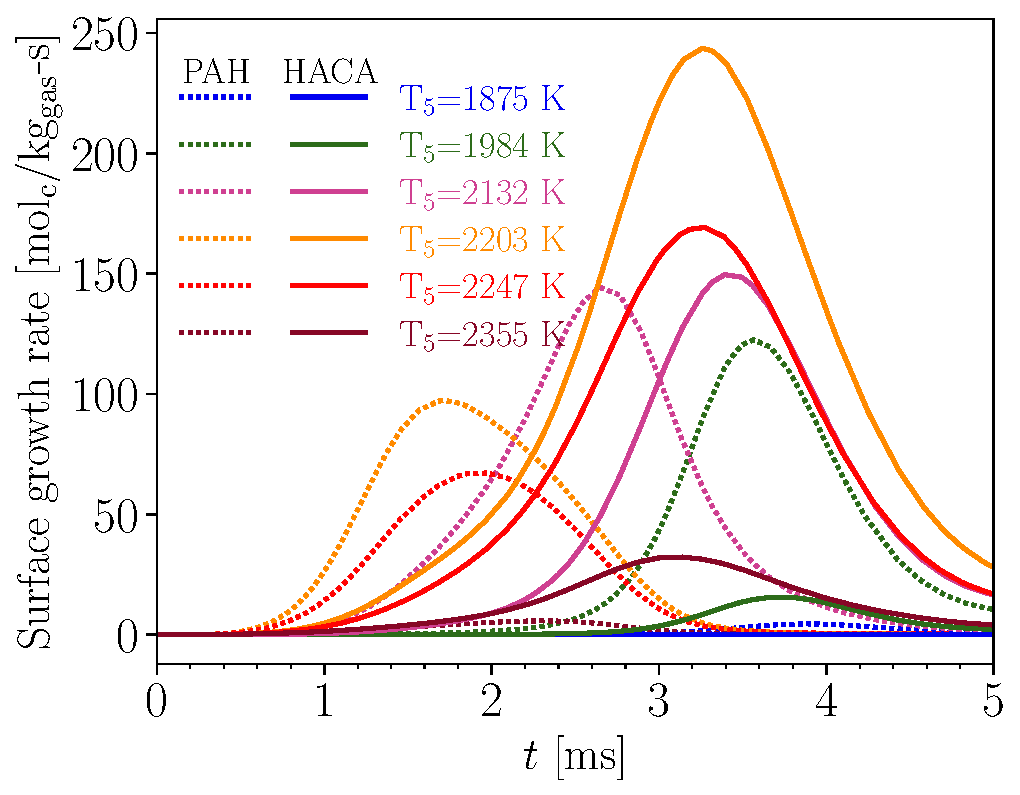
\includegraphics[width=0.45\textwidth]{Figures/time_growth.pdf}
	\caption{The CB surface growth rate via PAH adsorption (dashed line) and HACA (solid line) for different test conditions.}
	\label{fig:time_growth} 
\end{figure}

\begin{figure}[H]
	\centering
	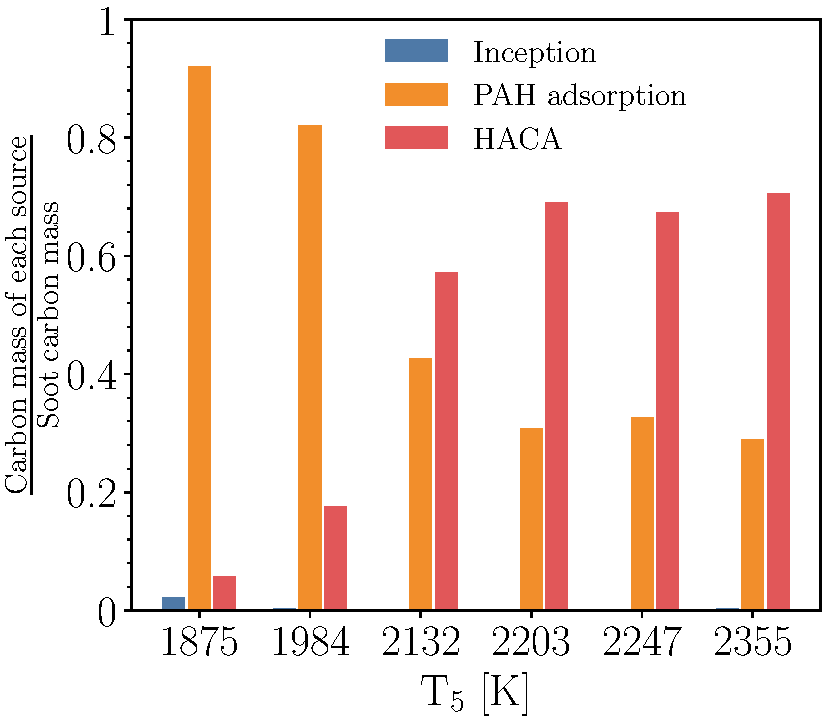
\includegraphics[width=0.45\textwidth]{Figures/carbon_cont.pdf}
	\caption{The CB mass from inception, PAH adsorption and HACA normalized by total carbon mass at $t$=5~ms}
	\label{fig:carbon_cont} 
\end{figure}